\documentclass{beamer}
% \documentclass[draft]{beamer}
\graphicspath{ {../figures/} }

% \includeonlyframes{frame3}

% Set the theme
\usetheme{Berlin}
% Remove navigation symbols for a cleaner look
\setbeamertemplate{navigation symbols}{}

% Title slide information
\title{Quantum State Discrimination}
\subtitle{A Demonstration of Related Works}
\author{Chien-Kai Ma}
\institute{NTU GIEE}
\date{May 15, 2025}

% For including images (uncomment if you add an image file)
% \usepackage{graphicx}
\usepackage{quantikz}
\usepackage[edges]{forest}
\usepackage{nccmath}
\usepackage{pgfplots}
\pgfplotsset{compat=1.18}

\forestset{
  direction switch/.style={
    for tree={edge+=thick, font=\sffamily},
    where level>=1{folder, grow'=0}{for children=forked edge},
    where level=3{}{draw},
  },
}

\usetikzlibrary{shapes.geometric, arrows}

\tikzstyle{startstop} = [rectangle, rounded corners, 
minimum width=3cm, 
minimum height=1cm,
text centered, 
text width=3cm,
draw=black, 
fill=red!30]

\tikzstyle{io} = [trapezium, 
trapezium stretches=true, % A later addition
trapezium left angle=70,
trapezium right angle=110,
minimum width=3cm,
minimum height=1cm,
align=center,
text width=5cm,
text centered,
draw=black, fill=blue!30]

\tikzstyle{process} = [rectangle, 
minimum width=3cm, 
minimum height=1cm, 
text centered, 
text width=4cm,
draw=black, 
fill=orange!30]

\tikzstyle{decision} = [diamond, 
minimum width=3cm, 
minimum height=1cm, 
text width=4cm,
aspect=2,
inner sep=-1ex,
text centered, 
draw=black, 
fill=green!30]
\tikzstyle{arrow} = [thick,->,>=stealth]

% Start the document
\begin{document}

% Title slide
\begin{frame}
  \titlepage
\end{frame}

% Table of Contents slide
\begin{frame}
  \frametitle{Table of Contents}
  \tableofcontents
\end{frame}


\section{Progress This Week}
\begin{frame}
  \frametitle{Main Algorithm -- Searching for a POVM for UQSD}
  \begin{center}
    \scalebox{0.45}{
      \usetikzlibrary{shapes.geometric, arrows}

\tikzstyle{startstop} = [rectangle, rounded corners,
minimum width=3cm,
minimum height=1cm,
text centered,
text width=3cm,
draw=black,
fill=red!30]

\tikzstyle{io} = [trapezium,
trapezium stretches=true, % A later addition
trapezium left angle=70,
trapezium right angle=110,
minimum width=3cm,
minimum height=1cm,
align=center,
text width=5cm,
text centered,
draw=black, fill=blue!30]

\tikzstyle{process} = [rectangle,
minimum width=3cm,
minimum height=1cm,
text centered,
text width=4cm,
draw=black,
fill=orange!30]

\tikzstyle{decision} = [diamond,
minimum width=3cm,
minimum height=1cm,
text width=4cm,
aspect=2,
inner sep=-1ex,
text centered,
draw=black,
fill=green!30]
\tikzstyle{arrow} = [thick,->,>=stealth]

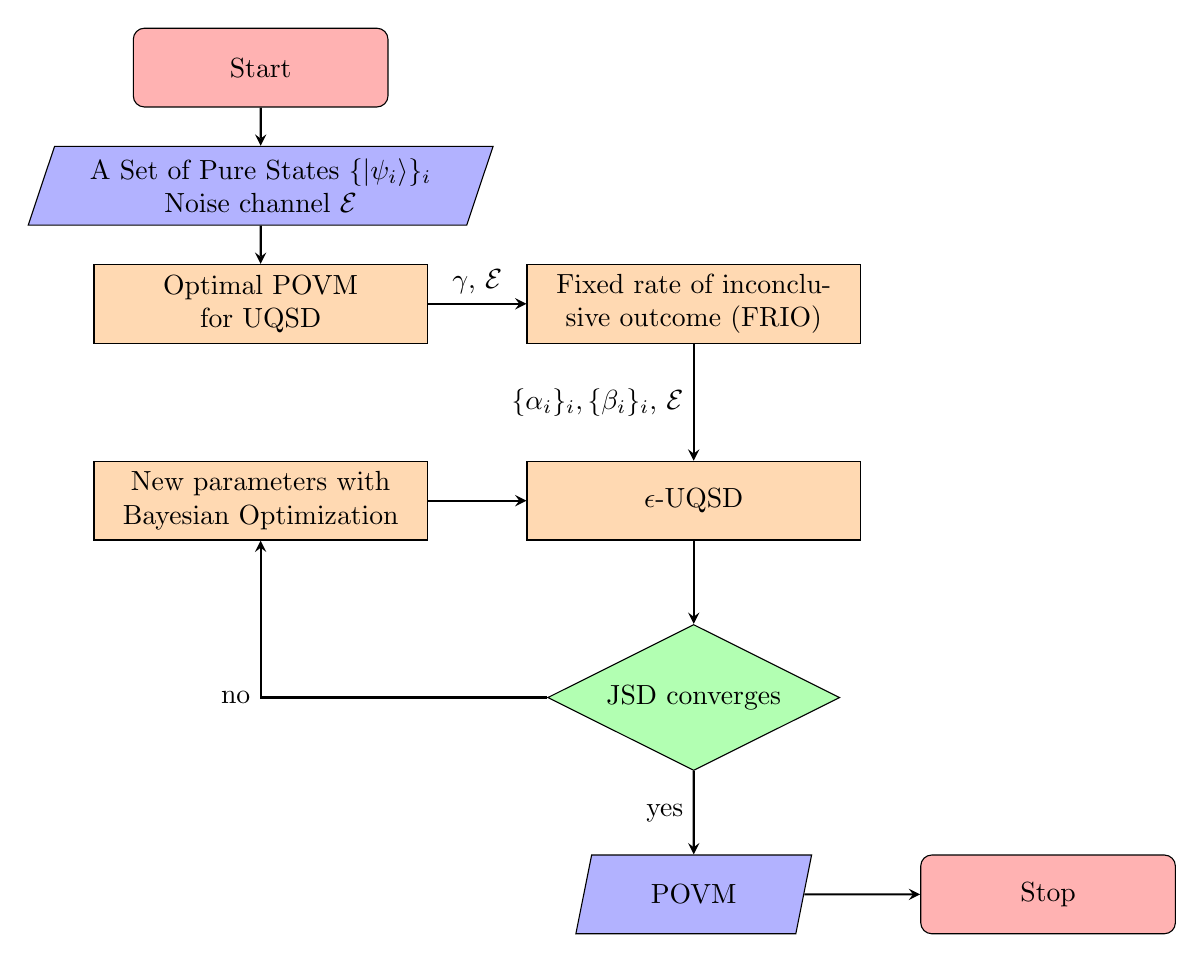
\begin{tikzpicture}[node distance=1.5cm]

    \node (start) [startstop] {Start};
    \node (in1) [io, below of=start] {%
        A Set of Pure States $\{\ket{\psi_{i}}\}_{i}$\\
        Noise channel $\mathcal{E}$\\
    };

    \node (pro1) [process, below of=in1] {
        Optimal POVM for UQSD\\
    };

    \node (pro2) [process, right of=pro1, xshift=4cm] {
        Fixed rate of inconclusive outcome (FRIO)\\
    };

    \node (pro3) [process, below of=pro2, yshift=-1cm] {
        $\epsilon$-UQSD\\
    };
    \node (pro4) [process, left of=pro3, xshift=-4cm] {
        New parameters with\\
        Bayesian Optimization\\
    };

    \node (dec1) [decision, below of=pro3, yshift=-1cm] {JSD converges};
    \node (out1) [io, below of=dec1, yshift=-1cm, text width=2cm] {
        POVM
    };
    \node (stop) [startstop, right of=out1, xshift=3cm] {Stop};

    \draw [arrow] (start) -- (in1);
    \draw [arrow] (in1) -- (pro1);
    \draw [arrow] (pro1) -- node[anchor=south] {$\gamma$, $\mathcal{E}$} (pro2);
    \draw [arrow] (pro2) -- node[anchor=east] {$\{\alpha_{i}\}_{i}, \{\beta_{i}\}_{i}$, $\mathcal{E}$} (pro3);
    \draw [arrow] (pro3) -- (dec1);
    % \draw [arrow] (dec1) -- ++(-3,0) node[left] {no} |- (pro3.west);
    \draw [arrow] (dec1) -| node[left] {no} (pro4);
    \draw [arrow] (pro4) -- (pro3);
    \draw [arrow] (dec1) -- node[anchor=east] {yes} (out1);
    \draw [arrow] (out1) -- (stop);

\end{tikzpicture}
    }
  \end{center}
\end{frame}

\begin{frame}
  \frametitle{Bayesian Optimization}
  \begin{itemize}
    \item Exploitation
    \item Exploration
  \end{itemize}
\end{frame}

\begin{frame}
  \frametitle{A List of Metrics}
  \begin{itemize}
    \item Jensen-Shannon Divergence
    \item Why we choose these metrics
  \end{itemize}
\end{frame}

\begin{frame}
  \frametitle{Jensen-Shannon Divergence}
  \begin{itemize}
    \item The Jensen-Shannon divergence (JSD) is a symmetrized and smoothed version of the Kullback-Leibler divergence
          $D_{KL}(P\parallel Q)$.
    \item For discrete probability distributions $P$ and $Q$
          defined on the same sample space $\mathcal{X}$, the
          relative entropy from $Q$ to $P$ is defined to be
          \begin{align}
            D_{KL}(P \parallel Q) = \sum_{x \in \mathcal{X}} P(x) \log {\frac{P(x)}{Q(x)}}
          \end{align}
    \item The Jensen-Shannon divergence is then defined by
          \begin{align}
            JSD(P\parallel Q) = \frac{1}{2}D_{KL}(P\parallel M) + \frac{1}{2}D_{KL}(Q\parallel M)
          \end{align}
          where $M = \frac{1}{2}(P + Q)$ is a mixture distribution of
          $P$ and $Q$.\\
  \end{itemize}
  \tiny{Reference: Wikipedia}
\end{frame}

\begin{frame}
  \frametitle{Jensen-Shannon Distance}
  \begin{itemize}
    \item The Jensen-Shannon distance is the square root of the Jensen-Shannon divergence.
          \begin{align}
            \sqrt{\frac{1}{2}D_{KL}(P\parallel M) + \frac{1}{2}D_{KL}(Q\parallel M)}
          \end{align}
  \end{itemize}
  \tiny{Reference: SciPy}
\end{frame}

\begin{frame}
  \frametitle{Quantum Jensen-Shannon Divergence}
  \begin{itemize}
    \item The generalization of probability distributions on density matrices allows to define
          quantum Jensen-Shannon divergence (QJSD).
    \item It is defined for a set of density matrices
          $(\rho_{1}, \dots, \rho_{n})$ and a probability distribution
          $\pi = (\pi_{1}, \dots, \pi_{n})$ as
          \begin{align}
            QJSD(\rho_{1}, \dots, \rho_{n}) = S(\sum_{i=1}^{n} \pi_{i} \rho_{i})
            - \sum_{i=1}^{n} \pi_{i} S(\rho_{i})
          \end{align}
          where $S{\rho}$ is the von Neumann entropy of $\rho$.
    \item This quantity is also called
          Holevo information, which gives the upper bound for the amount of
          classical information encoded by the quantum states $(\rho_{1}, \dots, \rho_{n})$
          under the prior distribution $\pi$.
  \end{itemize}
  \tiny{Reference: Wikipedia}
\end{frame}

\begin{frame}
  \frametitle{Bures metric/Helstrom metric}
  \begin{itemize}
    \item This metric defines an infinitesimal distance
          between denstiy matrix operators defining quantum states.
    \item The Bures metric may be defined as
          \begin{align}
            [ D_{B}(\rho, \rho+d\rho)]^{2} = \frac{1}{2}\operatorname{tr}(d\rho G)
          \end{align}
          where $G$ is the Hermitian 1-form operator implicitly given by
          \begin{align}
            \rho G + G \rho = d\rho
          \end{align}
  \end{itemize}
\end{frame}


\subsection{Solvers}
\begin{frame}
  \frametitle{Solve SDP with CVXPY}
  \begin{itemize}
    \item CVXPY is an open source Python-embedded modeling language for
          convex optimization problems.
    \item It lets you express your problem in a natural way that follows
          the math, rather than in the restrictive standard form required
          by solvers.
    \item Since semidefinite programming problems is a subset of convex
          optimization problems, it is natural for us to use this package.
    \item CVXPY relies on many open-source solvers like Clarabel, OSQP, and
          SCS, and it also supports additional solvers like CVXOPT, GLPK,
          and IBM CPLEX.
  \end{itemize}

  \tiny{Reference: \url{https://www.cvxpy.org/}}
\end{frame}

\begin{frame}
  \frametitle{Select a solver for CVXPY -- SCS}
  \begin{itemize}
    \item SCS (Splitting Conic Solver) is a numerical optimization package
          for solving large-scale convex quadratic cone problems.
    \item SCS can solve primal problems in the form of\\
          \begin{align}
             & \text{minimize}   &  & (1/2)x^{T} Px + c^{T}x \\
             & \text{subject to} &  & Ax + s = b             \\
             &                   &  & s \in \mathcal{K}
          \end{align}
          where $x \in \mathbf{R}^{n}$ is the primal variable,
          $s \in \mathbf{R}^{m}$ is the slack variable,
          $A \in \mathbf{R}^{m \times n}$,
          $b \in \mathbf{R}^{m}$,
          $P \in \mathbf{S}^{n}_{+}$,
          $c \in \mathbf{R}^{n}$,
          $\mathcal{K} \subseteq \mathbf{R}^{m}$
  \end{itemize}
\end{frame}

\begin{frame}
  \frametitle{Accelerate SCS with oneMKL}
  \begin{itemize}
    \item
    \item Intel® oneAPI Math Kernel Library (oneMKL)
    \item MKL is typically faster than the SCS's built-in linear system solver.
  \end{itemize}
  \tiny{Reference: https://www.cvxgrp.org/scs/install/python.html\#python-install}{Python - SCS documentation}
\end{frame}

\begin{frame}
  \frametitle{Accelerate solving SDP with CVXPY -- DPP}
  \begin{itemize}
    \item In CVXPY, "parameters" are symbolic representations of constants.
          Using parameters lets you modify the values of constants
          without reconstructing the entire problem.
    \item When your parametrized problem is constructed according to
          Disciplined Parametrized Programming (DPP), solving it repeatedly
          for different values of the parameters can be much faster than
          repeatedly solving a new problem.
  \end{itemize}
  \tiny{Reference: https://www.cvxpy.org/tutorial/dpp/index.html}
\end{frame}

\begin{frame}
  \frametitle{Verify that our problem can be transformed to DPP}
  \begin{itemize}
    \item (TODO) By checking the message of the solver, we verified that our problem
          can be parametrized and improved.
  \end{itemize}
  Your problem has 16384 variables, 20486 constraints, and 0 parameters.
  It is compliant with the following grammars: DCP, DQCP
\end{frame}


% Section 1: Introduction
\section{Introduction}
\begin{frame}
  \frametitle{Introduction to the Topic}
  \begin{itemize}
    \item<1-> This presentation demonstrates the progress of single-shot quantum state discrimination.
    \item<2-> We'll cover quantum state discrimination, theories, and circuit transformation.
    \item<3-> Feel free to interrupt for questions!
  \end{itemize}
\end{frame}

\begin{frame}{Structure of My Research}
  \resizebox{\textwidth}{!}{
    \begin{forest}
      direction switch
        [QSD Project Organization
            [Quantum State Discrimination
                [Pure states
                    [Demonstration of UD in circuits]
                ]
                [Mixed states
                    [QD with FRIO]
                    [$\epsilon$-Unambiguous discrimination]
                ]
                [IPFS Dapp
                    [Drizzle Truffle]
                    [Solidity Contract]
                    [Deploy to Surge]
                ]
            ]
            [Academic
                [ENGR Year 4
                    [CENG 4B]
                    [CENG 4A]
                ]
                [Tutorials
                    [Voting Dapp]
                ]
                [Article Summary
                    [Vyper + Truffle]
                    [Tensorflow]
                    [HashGraph]
                ]
            ]
            [Quantum Circuit
                [Exact synthesis]
                [Approximate synthesis]
                [Ideal simulation]
                [Noisy simulation]
            ]
            [Applications
                []
                []
            ]
            [Results and Comparisons
                []
            ]
        ]
    \end{forest}
  }
\end{frame}

% \begin{frame}{Structure of Relevant Research Topics}
%   \resizebox{\textwidth}{!}{
%     \begin{forest}
%       direction switch
%       [Relevant Topics
%       [Quantum Detection
%       [Hypothesis testing
%       ]
%       [Vue-Dapp
%       [Docsaurus]
%       [Deploy to MainNet]
%       [Update Todolist]
%       ]
%       [IPFS Dapp
%         [Drizzle Truffle]
%         [Solidity Contract]
%         [Deploy to Surge]
%       ]
%       ]
%       [Academic
%         [ENGR Year 4
%             [CENG 4B]
%             [CENG 4A]
%         ]
%         [Tutorials
%             [Voting Dapp]
%         ]
%         [Article Summary
%             [Vyper + Truffle]
%             [Tensorflow]
%             [HashGraph]
%         ]
%       ]
%       [Quantum Measurement
%         [POVM]
%         []
%       ]
%       [Quantum Circuit
%         [Exact synthesis]
%         [Approximate synthesis]
%         [Ideal simulation]
%         [Noisy simulation]
%       ]
%       [Applications
%         [Quantum resource theory]
%         [Quantum key distribution]
%         [Quantum state tomography]
%       ]
%       ]
%     \end{forest}
%   }
% \end{frame}


\section{The Evolution}


\begin{frame}
  \frametitle{Evolution of the Topic}
  \begin{itemize}
    \item<1-> "Testing of Simple Hypotheses by a Single Measurement" (Helstrom, 1969)
    \item<2->
    \item<3->
  \end{itemize}
\end{frame}

\begin{frame}
  \frametitle{Quantum Hypothesis Testing}
  \begin{columns}[T] % T aligns tops of columns
    \begin{column}{0.5\textwidth}
      \begin{block}{Definition}
      \end{block}
    \end{column}
    \begin{column}{0.5\textwidth}
      \begin{alertblock}{Important Note}
        Use \texttt{alertblock} for emphasis!
      \end{alertblock}
    \end{column}
  \end{columns}
\end{frame}

\begin{frame}
  \frametitle{Naimark's theorem}
\end{frame}

\subsection{Theoretical Bounds}
\begin{frame}
  \frametitle{Quantum Chernoff bound}
\end{frame}

\begin{frame}
  \frametitle{Holevo bound}
\end{frame}
\begin{frame}{Abbreviations}
  \begin{description}
    \item[QSD] Quantum state discrimination
    \item[MED] Minimum-error discrimination
    \item[UD] Unambiguous discrimination
    \item[FRIO] Fixed rate of inconclusive outcomes
    \item[AOSD] Assisted optimal state discrimination
    \item[POVM] Positive operator-valued measure
    \item[PVM] Projective measurement
    \item[PGM] Pretty good measurement
  \end{description}
\end{frame}

\section{Experimental Results}
\subsection{Discriminating two coherent states}
\begin{frame}
  \frametitle{<title>}
  Solving once is not always enough.
  We investigate in different orders to find a reasonable POVM for
  quantum state discrimination.
\end{frame}

\subsection{Discriminating pure quantum states with noise injection}


% Algorithm 1
\begin{frame}
  \frametitle{Main Algorithm - Searching for a POVM for UQSD}
  \begin{center}
    \scalebox{0.5}{
      \usetikzlibrary{shapes.geometric, arrows}

\tikzstyle{startstop} = [rectangle, rounded corners,
minimum width=3cm,
minimum height=1cm,
text centered,
text width=3cm,
draw=black,
fill=red!30]

\tikzstyle{io} = [trapezium,
trapezium stretches=true, % A later addition
trapezium left angle=70,
trapezium right angle=110,
minimum width=3cm,
minimum height=1cm,
align=center,
text width=5cm,
text centered,
draw=black, fill=blue!30]

\tikzstyle{process} = [rectangle,
minimum width=3cm,
minimum height=1cm,
text centered,
text width=4cm,
draw=black,
fill=orange!30]

\tikzstyle{decision} = [diamond,
minimum width=3cm,
minimum height=1cm,
text width=4cm,
aspect=2,
inner sep=-1ex,
text centered,
draw=black,
fill=green!30]
\tikzstyle{arrow} = [thick,->,>=stealth]

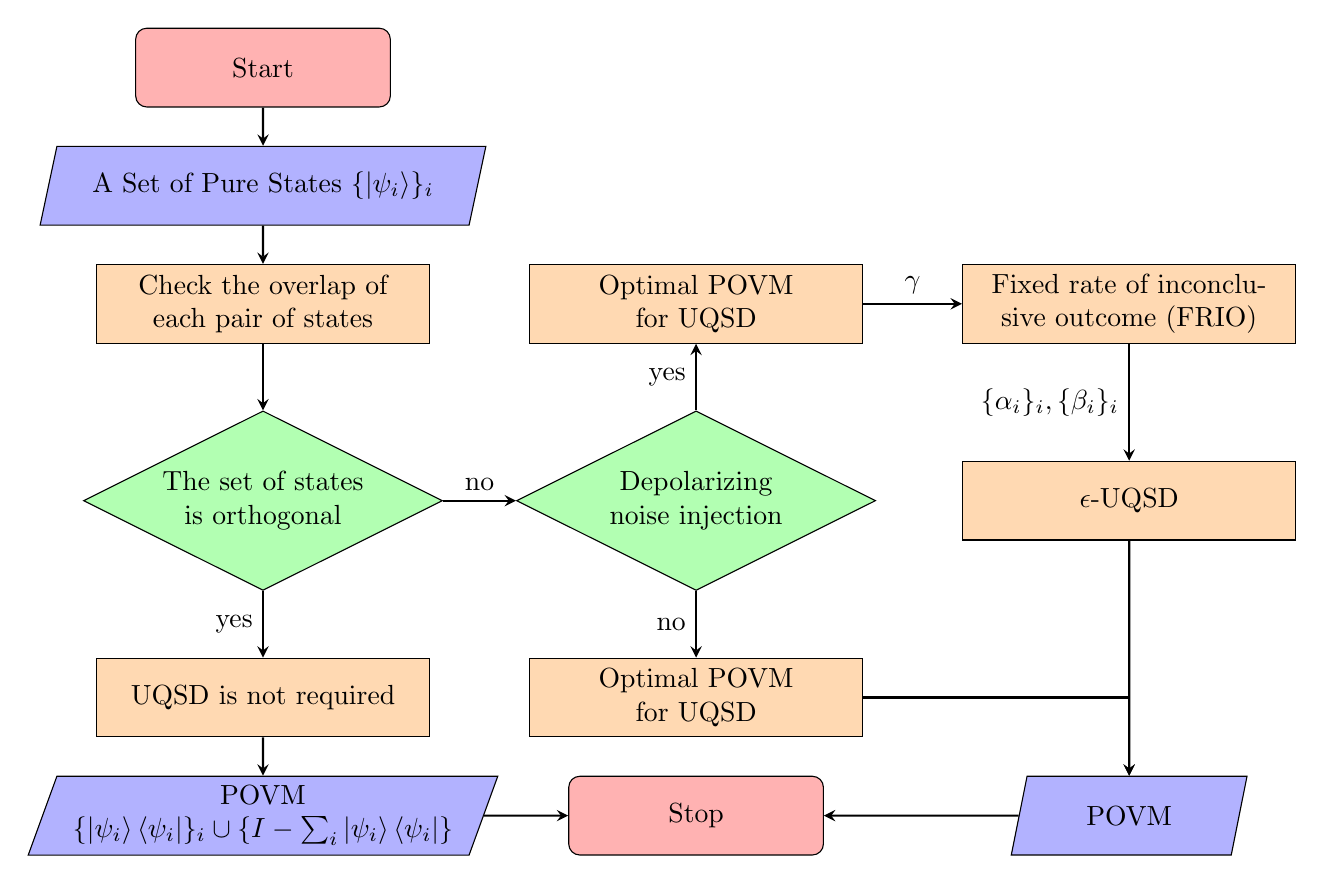
\begin{tikzpicture}[node distance=1.5cm]

    \node (start) [startstop] {Start};
    \node (in1) [io, below of=start] {%
    A Set of Pure States $\{\ket{\psi_{i}}\}_{i}$\\
    };
    \node (pro1) [process, below of=in1] {
        Check the overlap of each pair of states
    };
    \node (dec1) [decision, below of=pro1, yshift=-1cm] {
        The set of states is orthogonal
    };

    \node (pro2) [process, below of=dec1, yshift=-1cm] {
        UQSD is not required\\
    };

    \node (dec2) [decision, right of=dec1, xshift=4cm] {
        Depolarizing noise injection\\
    };

    \node (pro3) [process, below of=dec2, yshift=-1cm] {
        Optimal POVM for UQSD\\
    };

    \node (pro4a) [process, above of=dec2, yshift=1cm] {
        Optimal POVM for UQSD\\
    };
    \node (pro4b) [process, right of=pro4a, xshift=4cm] {
        Fixed rate of inconclusive outcome (FRIO)\\
    };
    \node (pro4c) [process, below of=pro4b, yshift=-1cm] {
        $\epsilon$-UQSD\\
    };
    \node (out1) [io, below of=pro2] {
    POVM\\
    $\{\ket{\psi_{i}}\bra{\psi_{i}}\}_{i} \cup \{I - \sum_{i}{\ket{\psi_{i}}\bra{\psi_{i}}}\}$
    };
    \node (stop) [startstop, right of=out1, xshift=4cm] {Stop};
    \node (out2) [io, right of=stop, xshift=4cm, text width=2cm] {
        POVM
    };

    \draw [arrow] (start) -- (in1);
    \draw [arrow] (in1) -- (pro1);
    \draw [arrow] (pro1) -- (dec1);
    \draw [arrow] (dec1) -- node[anchor=east] {yes} (pro2);
    \draw [arrow] (dec1) -- node[anchor=south] {no} (dec2);
    \draw [arrow] (dec2) -- node[anchor=east] {no} (pro3);
    \draw [arrow] (dec2) -- node[anchor=east] {yes} (pro4a);
    \draw [arrow] (pro4a) -- node[anchor=south] {$\gamma$} (pro4b);
    \draw [arrow] (pro4b) -- node[anchor=east] {$\{\alpha_{i}\}_{i}, \{\beta_{i}\}_{i}$} (pro4c);
    \draw [arrow] (pro4c) -- (out2);
    \draw [arrow] (pro3) -| (out2);
    \draw [arrow] (pro2) -- (out1);
    \draw [arrow] (out1) -- (stop);
    \draw [arrow] (out2) -- (stop);

\end{tikzpicture}
    }
  \end{center}
\end{frame}

% Formulation of each problems?
\begin{frame}[label=frame0]
  \frametitle{Optimal POVM for UQSD}
  % Add reference and some introductions
  \begin{itemize}
    \item Calculate reciprocal states $\{\ket{\tilde{\psi_{i}}}\}$, which lead to the Hermitian operators $\{\Pi_{i}\}$
    \item $\Pi_{i} = \ket{\tilde{\psi_{i}}}\bra{\tilde{\psi_{i}}} \succeq 0, \quad i = 1, \ldots, k$
    \item Solve SDP for the coefficients of the measurement operators ($\{x_{i}\}$)
          \begin{align}
             & \underset{\{x_{i}\}}{\text{maximize}} &  & P_{D}=\sum_{i=1}^{k} p_{i} x_{i}           \\
             & \text{subject to}                     &  & I - \sum_{i=1}^{k} x_{i} \Pi_{i} \succeq 0
          \end{align}
  \end{itemize}
\end{frame}

\begin{frame}[label=frame4]
  \frametitle{Fixed Rate of Inconclusive Outcome (FRIO)}
  \begin{itemize}
    \item A quantum state $\Psi$ can be denoted by a state vector $\ket{\psi}$ or a density matrix $\rho$.
          The prior probability for each input state $\Psi_{i}$ (expressed by $\ket{\psi_{i}}$ or $\rho_{i}$) is
          denoted by $p_{i}$, where $i$ ranges from 1 to $k$.
          The measurement operators are defined by $\Pi_{i}$, where $i$ ranges from 0 to $k$.
    \item Here $\Pi_{0}$ is designed to match the inconclusive results,
          and $\Pi_{1}$ to $\Pi_{k}$ designed to measure the $1$-st to $k$-th state respectively.
          $P_{D}$ denotes the total probability of correct discrimination,
          $P_{err}$ denotes the probability of incorrect/erroneous discrimination,
          and $P_{inc}$ denotes the probability of inconclusive outcomes.
          $\beta$ is a constant real number that is defined to be the target inconclusive probability.
  \end{itemize}
  % Add reference and some introductions

\end{frame}

\begin{frame}
  \frametitle{Fixed Rate of Inconclusive Outcome (FRIO)}
  \begin{itemize}
    \item In practice, we use an inequality in place of an equality,
          and $\beta$ is the minimum rate of inconclusive outcomes.
    \item The semidefinite programming formulation
          \begin{align}
             & \underset{\{\Pi\}}{\text{maximize}} &  & P_{D}=\sum_{i=1}^{k} p_{i} \operatorname{Tr}(\rho_{i} \Pi_{i})              \\
             & \text{subject to}                   &  & \Pi_{i} \succeq 0, \quad i = 0, \ldots, k                                   \\
             &                                     &  & \sum_{i=0}^{k} \Pi_i = I                                                    \\
             &                                     &  & P_{inc}=\sum_{i=1}^{k} p_{i} \operatorname{Tr}(\rho_{i} \Pi_{0}) \geq \beta
          \end{align}
  \end{itemize}
\end{frame}

\begin{frame}
  \frametitle{$\epsilon$-UQSD}
  % TODO Add explanations
  Some explanations and definitions
\end{frame}

\begin{frame}
  \frametitle{$\epsilon$-UQSD}
  % Add reference and some introductions
  \begin{align}
     & \underset{\{\Pi\}}{\text{maximize}} &  & P_{D}=\sum_{i=1}^{k} p_{i} \operatorname{Tr}(\rho_{i} \Pi_{i})                                                                                                      \\
     & \text{subject to}                   &  & \Pi_{i} \succeq 0, \quad i = 0, \ldots, k                                                                                                                           \\
     &                                     &  & \sum_{i=0}^{k} \Pi_i = I                                                                                                                                            \\
     &                                     &  & P(O_i \mid \rho_i) = \frac{p_i \, \operatorname{Tr}(\rho_i \Pi_i)}{\sum_{j=1}^{L} p_i \, \operatorname{Tr}(\rho_i \Pi_j)} \geq 1 - \alpha_i, \quad i = 1, \ldots, k \\
     &                                     &  & P(\rho_i \mid O_i) = \frac{p_i \, \operatorname{Tr}(\rho_i \Pi_i)}{\sum_{j=1}^{L} p_j \, \operatorname{Tr}(\rho_j \Pi_i)} \geq 1 - \beta_i, \quad i = 1, \ldots, k
  \end{align}
\end{frame}

%% \begin{frame}
%%   \frametitle{Overlap and state fidelity}
%% 
%% 
%% \end{frame}

\begin{frame}
  \frametitle{UQSD of Coherent States}
  \begin{itemize}
    \item "Adaptive Generalized Measurement for Unambiguous
          State Discrimination of Quaternary Phase-Shift-Keying
          Coherent States"
    \item The work discussed UQSD of 4 coherent evenly spread
          around the x-p diagram
  \end{itemize}
\end{frame}

\begin{frame}
  \frametitle{Canonical Coherent States}
  The canonical coherent states have three properties that are mutually equivalent (wiki, TODO rewrite?)
  \begin{itemize}
    \item They are eigenvectors of the annihilation operator: $\hat{a}\ket{\alpha}=\alpha\ket{\alpha}$
    \item They are obtained from the vacuum by application of a unitary displacement operator:
          $\ket{\alpha}=(e^{\alpha \hat{a}^{\dagger} - \alpha^{*}\hat{a}})\ket{0}=D(\alpha)\ket{0}$
    \item They are states of minimal uncertainty: $\Delta{X} = \Delta{P} = \sqrt{\frac{\hbar}{2}}$
  \end{itemize}
\end{frame}

\begin{frame}
  \frametitle{Demo - State Selection}
  \begin{itemize}
    \item Truncated coherent states and fidelity is important...
          We chose the following three sets of coherent states to demonstrate the dynamics of
          the different methods to search for a proper POVM for state discrimination.
    \item First, we want the set of coherent states to show some symmetric property.
          Since each coherent state correspond to an annihilation operator with a unique eigenvalue,
          we set the eigenvalues to have the same magnitude but different angles and the difference of
          each pair of angles is the same. We can visualize the states with Wigner function, as the figure below.
  \end{itemize}
\end{frame}

\begin{frame}
  \frametitle{Influence of Truncation of Coherent States}
  \begin{center}
    \scalebox{0.2}{
      \includegraphics{../figures/trun_coh.png}
    }
  \end{center}
\end{frame}

\begin{frame}
  \frametitle{Influence of Truncation of Coherent States}
  \begin{itemize}
    \item We also calculated the fidelity of truncated
          coherent states by padding zeros to the same dimension.
    \item A truncated coherent state with the largest dimension
          is selected as the reference.
    \item So for $\alpha = 4$, we will select $N = 64$.
  \end{itemize}
  \begin{table}[ht]
    \centering
    \scalebox{0.6}{
      \begin{tabular}{r r}
        \hline
        \textbf{Fock States (N)} & \textbf{Fidelity}    \\
        \hline
        2                        & 1.525e-06            \\
        4                        & 5.193e-07            \\
        8                        & 2.606e-04            \\
        16                       & 2.674e-01            \\
        32                       & 0.999594             \\  % ← This is the special one
        64                       & 1.0 (0 to 13 digits) \\
        128                      & 1.0 (0 to 13 digits) \\
        256                      & 1.0 (0 to 13 digits) \\
        512                      & 1.0 (0 to 13 digits) \\
        1024                     & 1.0 (0 to 13 digits) \\
        \hline
      \end{tabular}
    }
    \caption{Fidelity of $\ket{\alpha}$ w.r.t N = 1024 ($\alpha = 4$)}
    \label{tab:fock-fidelity}
  \end{table}
\end{frame}

\begin{frame}
  \frametitle{Selecting $\alpha$}
  \begin{itemize}
    \item It is also important to choose $\alpha$ (The eigenvalue of the
          annihilation operator).
    \item Since we know the closed form of coherent states, we can evaluate
          the overlap before we decide the sets of states.
  \end{itemize}
\end{frame}

\begin{frame}
  \frametitle{Theoretical overlap of canonical coherent states}
  \begin{center}
    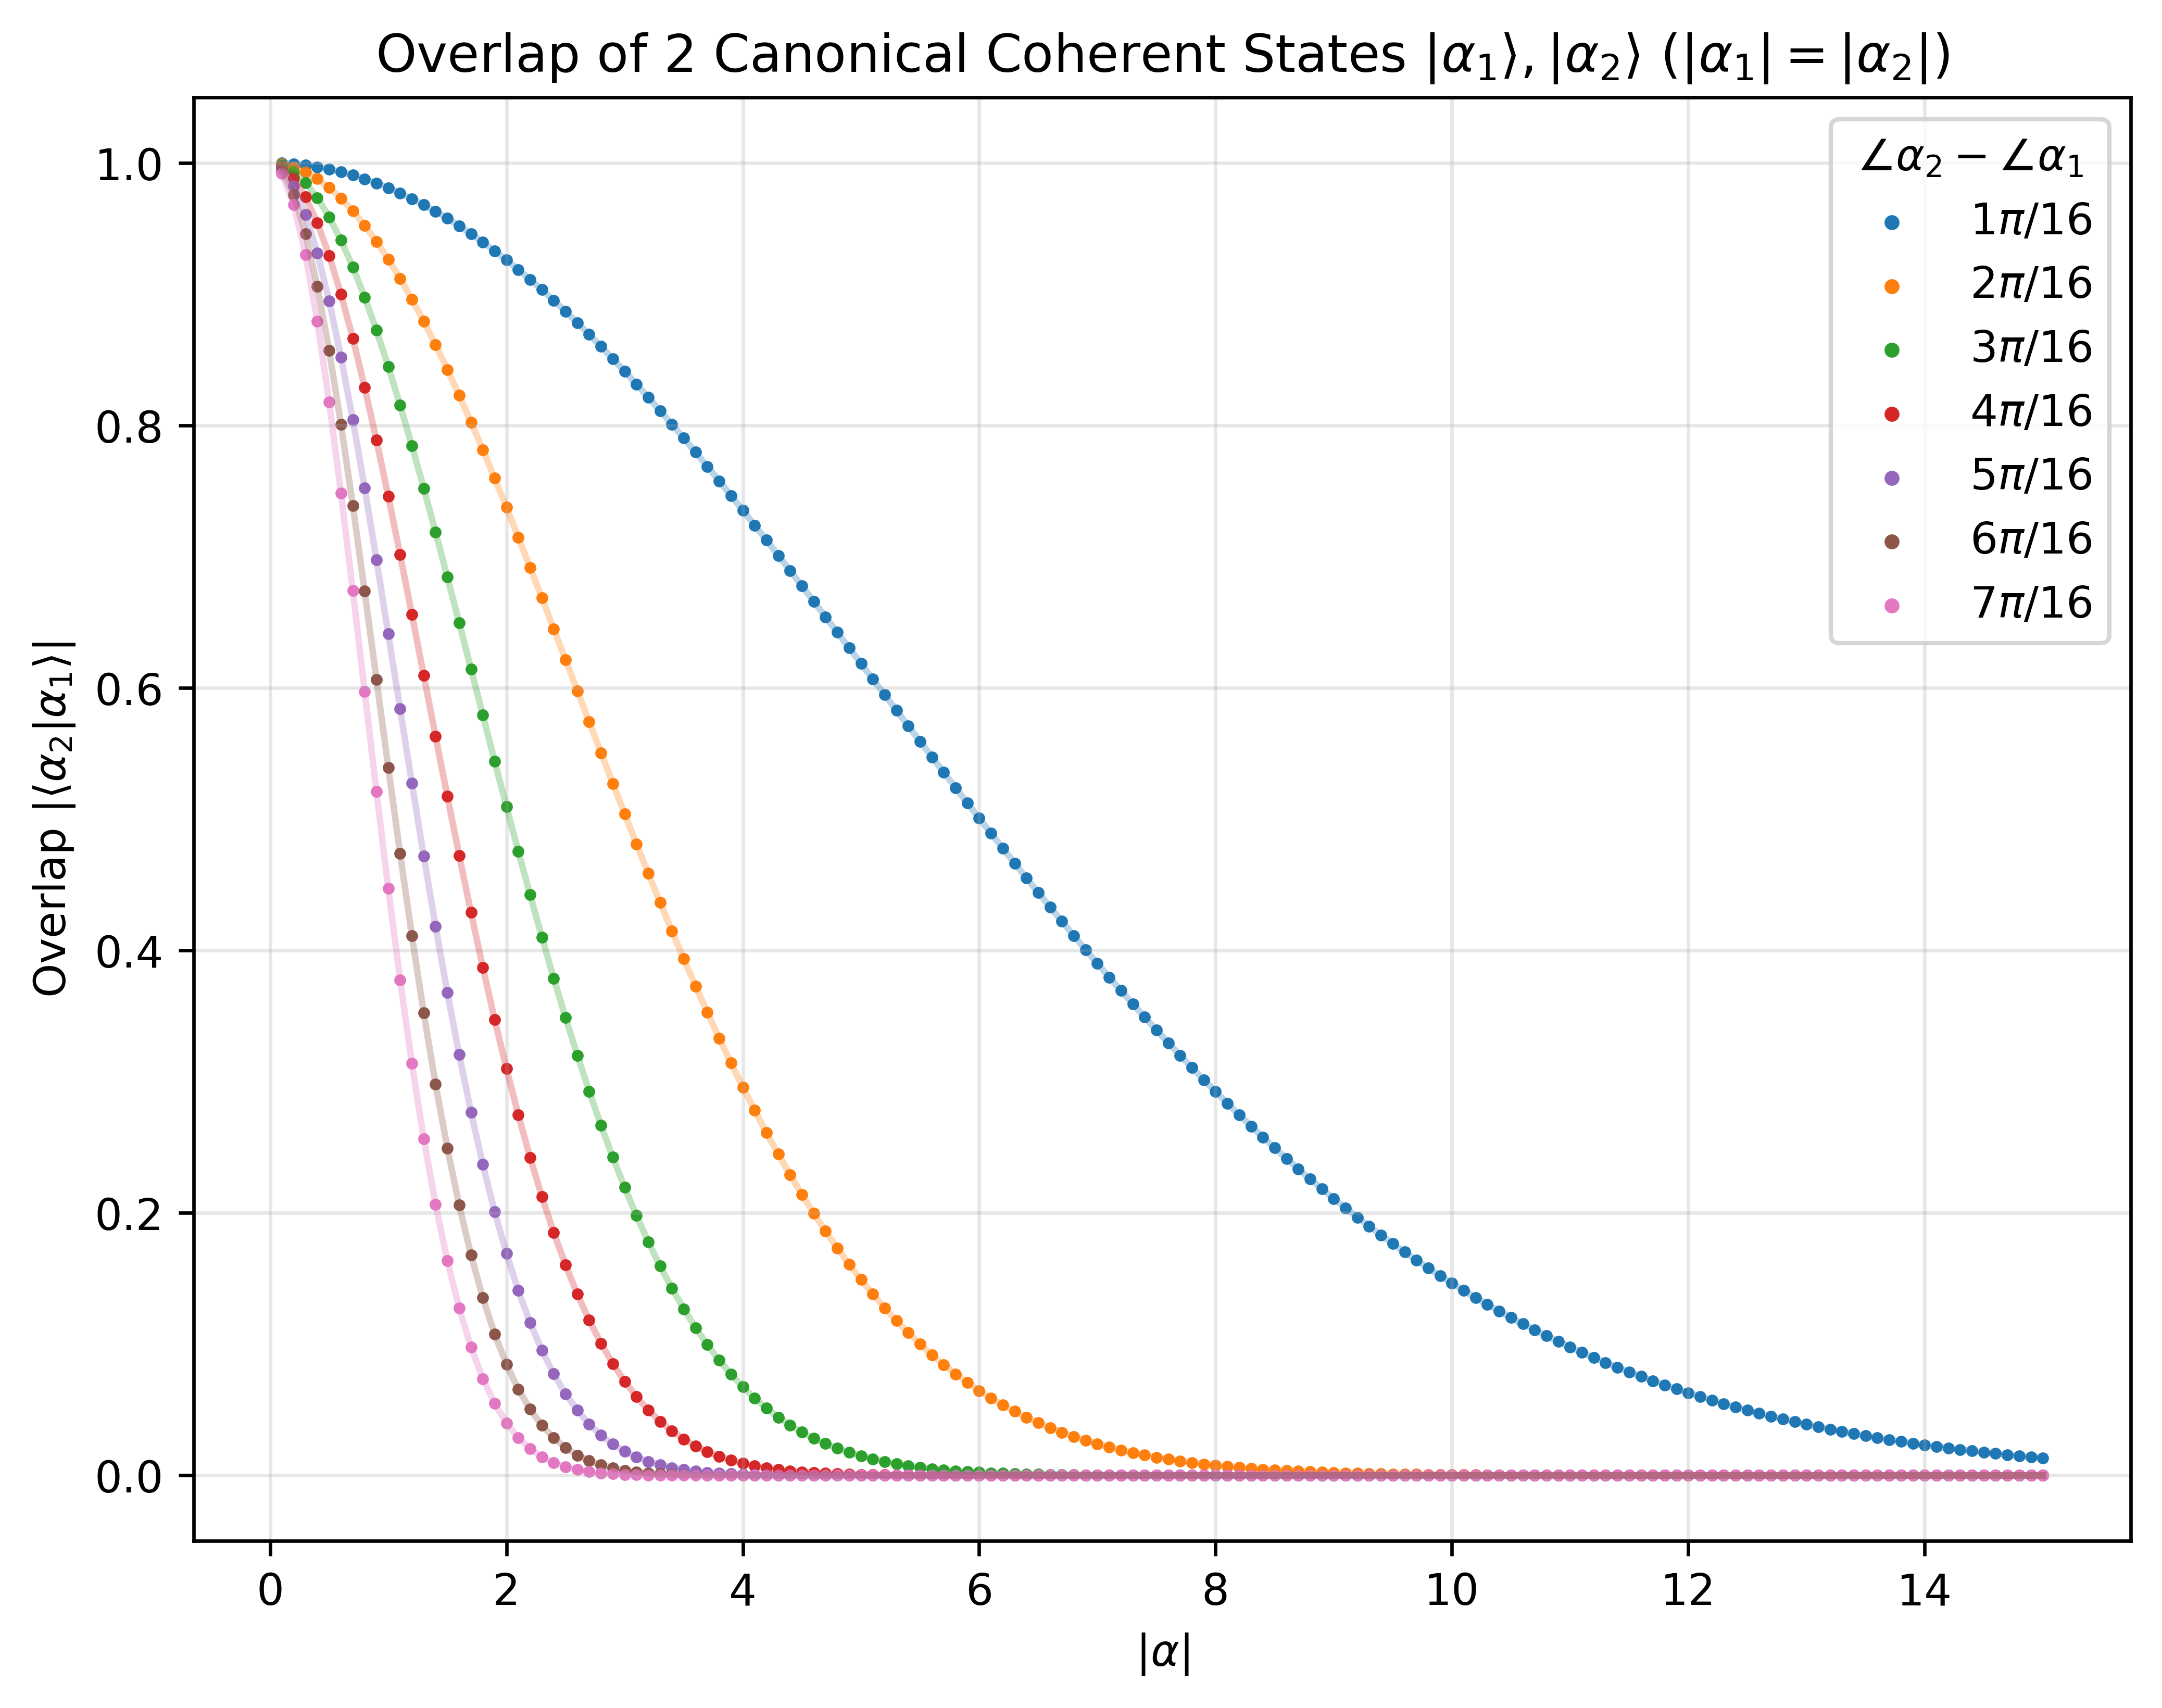
\includegraphics[width=0.7\textwidth]{../figures/overlap.png}
  \end{center}
\end{frame}

\begin{frame}
  \frametitle{Theoretical overlap of canonical coherent states}
  For two different canonical coherent states $\ket{\alpha}$ and $\ket{\beta}$,
  \begin{align}
    \braket{\beta}{\alpha} = e^{-\frac{1}{2}(|\beta|^{2} + |\alpha|^{2} - 2\beta^{*}\alpha)}
  \end{align}

  Assume $\alpha = r_{1}e^{i\theta_{1}}$, $\beta = r_{2}e^{i\theta_{2}}$,
  \begin{align}
    \braket{\beta}{\alpha} = e^{-\frac{1}{2}(r_{1}^{2} + r_{2}^{2} - 2r_{1}r_{2}e^{i(\theta_{1}-\theta_{2})})}
  \end{align}

  If $r_{1} = r_{2} = r$,
  \begin{align}
    \braket{\beta}{\alpha} = e^{-r^{2}(1 - e^{i(\theta_{1}-\theta_{2})})}
  \end{align}

  If $\theta_{1} = \theta_{2} = \theta$,
  \begin{align}
    \braket{\beta}{\alpha} = e^{-\frac{1}{2}(r_{1} - r_{2})^{2}}
  \end{align}
\end{frame}

\begin{frame}
  \frametitle{$\epsilon$-UQSD of Coherent States}
  \begin{itemize}
    \item Current problem
    \item It takes very long (>20 minutes on my laptop)
          to find the solution.
  \end{itemize}
\end{frame}

% \begin{center}
%   \scalebox{0.7}{
%     \begin{tikzpicture}
%       \begin{axis}[
%           xlabel={Number of Fock states in Hilbert space},
%           ylabel={Fidelity},
%           xmode=log,
%           log basis x=2,
%           xtick=data,
%           enlargelimits=0.1,
%           width=10cm,
%           height=6cm,
%           grid=major,
%           log basis y=10,
%           nodes near coords,
%           point meta=explicit symbolic,
%           every node near coord/.style={
%               anchor=south,
%               font=\scriptsize,
%               xshift=0pt,
%               yshift=-8pt
%             }
%         ]
%         \addplot+ coordinates {
%             (2, 1.5247e-6)  [ ]
%             (4, 5.1925e-7)  [ ]
%             (8, 0.0002606)  [ ]
%             (16, 0.267448)  [ ]
%             (32, 0.999594)  [0.999594]
%             (64, 1.0)       [ ]
%             (128, 1.0)      [ ]
%             (256, 1.0)      [ ]
%             (512, 1.0)      [ ]
%             (1024, 1.0)     [ ]
%           };
%       \end{axis}
%     \end{tikzpicture}
%   }
% \end{center}
% 
\section{Applications}
\begin{frame}
  \frametitle{Applications}
  \begin{itemize}
    \item Quantum key distribution
    \item Quantum teleportation
    \item Quantum tomography
    \item Exoplanet detection
    \item Quadrature Phase Shift Keying (QPSK)
          Increasing communication bandwidth
    \item Quantum random number generation
    \item Quantum illumination
  \end{itemize}
\end{frame}

\begin{frame}
  \frametitle{Details of the Applications}



\end{frame}

\section{Problem Formulation}
\begin{frame}
  \frametitle{Our Motivation}
  Our motivation was to investigate the behavior of UQSD in the presence
  of quantum noises. We tried to translate the POVM to a quantum circuit
  with Naimark's theorem, and ...
\end{frame}

\section{Methods}
\begin{frame}
  \frametitle{Postprocessing POVMs}
  \begin{itemize}
    \item The measurement operators obtained from CVXPY may not be rank-1.
    \item
  \end{itemize}
\end{frame}

% Section 5: Conclusion
\section{Conclusion}
\begin{frame}
  \frametitle{Summary}
  \begin{itemize}
    \item We've explored columns, blocks, overlays, and tables.
    \item Beamer is highly customizable for professional presentations.
  \end{itemize}
  \vfill
  \begin{center}
    \alert{Thank you for your attention!}
  \end{center}
\end{frame}

\section{SIC-POVM}
\begin{frame}
  \frametitle{Definitions on Wikipedia}
  \begin{block}{POVM}
    A POVM over a \textit{d}-dimensional Hilbert space $\mathcal{H}$ is a set of
    \textit{m} positive-semidefinite operators ${\{F_{i}\}^{m}_{i=1}}$ that sum to the identity:
    $\sum_{i=1}^{m}F_{i}=I$
  \end{block}
  \begin{block}{IC-POVM}
    If a POVM consists of at least $d^2$ operators which span the space of self-adjoint operators
    $\mathcal{L(H)}$, it is said to be an informationally complete POVM.
  \end{block}
  \begin{block}{Minimal IC-POVM}
    IC-POVMs consisting of exactly $d^2$ elements are called minimal.
  \end{block}
\end{frame}

\begin{frame}
  \frametitle{Definitions on Wikipedia}
  \begin{block}{SIC-POVM}
    A set of $d^2$ rank-1 projectors ${\{\Pi_{i}\}^{d^2}_{i=1}}$
    which have equal pairwise Hilbert-Schmidt inner products,
    $\textnormal{Tr} (\Pi_{i}\Pi_{j})=\frac{d\delta_{ij}+1}{d+1}$,\\
    defines a "minimal IC-POVM" with elements $F_{i}=\frac{1}{d}\Pi_{i}$
    called a SIC-POVM.
  \end{block}
  \begin{alertblock}{S in "SIC" stands for symmetric}
    Any pair of elements has the same Hilbert–Schmidt inner product as any other pair.
  \end{alertblock}
\end{frame}

\begin{frame}
  \frametitle{Example}
  % Selecting fiducial states that construct the projectors of SIC-POVMs
  \begin{block}{$d = 2$}
    $\ket{\psi_{1}} = \ket{0}$\\
    $\ket{\psi_{2}} = \frac{1}{\sqrt{3}}\ket{0} + \sqrt{\frac{2}{3}}\ket{1}$\\
    $\ket{\psi_{3}} = \frac{1}{\sqrt{3}}\ket{0} + \sqrt{\frac{2}{3}} e^{i\frac{2\pi}{3}}\ket{1}$\\
    $\ket{\psi_{4}} = \frac{1}{\sqrt{3}}\ket{0} + \sqrt{\frac{2}{3}} e^{i\frac{4\pi}{3}}\ket{1}$\\
  \end{block}
  \begin{itemize}
    \item Since a rank-1 operator can be uniquely defined by a vector, I will call these vectors the fiducial states.
  \end{itemize}
\end{frame}

\begin{frame}
  \frametitle{Unambiguous discrimination of fiducial states of SIC-POVMs}
  \begin{itemize}
    \item Since the states are linearly dependent, there is no non-trivial solution for unambiguous discrimination.
    \item For this set of states, even if you allow for some tolerance of error, the best solution is not be conclusive at all.
    \item Only when the tolerance is set to 0.5 (which is very ridiculous), you can obtain non-trivial measurement
          operators and the inconclusive result is 0.
    \item What if you don't use the corresponding SIC-POVM?
    \item What constraints make sense?
  \end{itemize}
\end{frame}

\begin{frame}
  \frametitle{Possible points}
  \begin{itemize}
    \item Even though the SIC-POVM seems to be best, it may not be the case
          under noisy conditions. Then maybe a slightly not perfect POVM may
          perform better.
    \item
  \end{itemize}
\end{frame}

\begin{frame}
  \frametitle{Every SIC-POVM is a 2-design}
  \begin{block}{Hyperspheres}
    In mathematics, an n-sphere or hypersphere is an ${\displaystyle
          n}$-dimensional generalization of the ${\displaystyle 1}$-dimensional
    circle and ${\displaystyle 2}$-dimensional sphere to any non-negative
    integer ${\displaystyle n}$. \\
    Given a Cartesian coordinate system, the unit ${\displaystyle n}$-sphere
    of radius ${\displaystyle 1}$ can be defined as: ${\displaystyle S^{n}=\left\{x\in \mathbb {R} ^{n+1}:
          \left\|x\right\|=1\right\}.}$
  \end{block}
  \begin{block}{Spherical t-designs}
    A spherical t-design is a set of vectors ${\displaystyle S=\left\{|\phi _{k}\rangle :|\phi _{k}\rangle \in \mathbb {S}
          ^{d}\right\}}$ on the d-dimensional generalized hypersphere, such that the
    average value of any ${\displaystyle t^{th}}$-order polynomial
    ${\displaystyle f_{t}(\psi )}$ over ${\displaystyle S}$ is equal to the
    average of ${\displaystyle f_{t}(\psi )}$ over all normalized
    vectors $\ket{\psi}$.
  \end{block}
\end{frame}

\begin{frame}
  \frametitle{Every SIC-POVM is a 2-design}
  Defining
  %${\displaystyle {\mathcal {H}}_{t}=\displaystyle \bigotimes _{i=1}^{t}{\mathcal {H}}}$ as the t-fold
  %tensor product of the Hilbert spaces, and
  ${\displaystyle S_{t}=\displaystyle \sum
        _{k=1}^{n}|\Phi _{k}^{t}\rangle \langle \Phi _{k}^{t}|,\quad |\Phi
        _{k}^{t}\rangle =|\phi _{k}\rangle ^{\otimes t}}$ as the t-fold tensor
  product frame operator,
  it can be shown that a set of normalized vectors
  ${\displaystyle \left\{|\phi _{k}\rangle \in
    \mathbb {S} ^{d}\right\}_{k=1}^{n}}$ with
  ${\displaystyle n\geq \binom{t+d-1}{d-1}}$ forms a spherical t-design if and
  only if ${\displaystyle \displaystyle \mathrm {Tr}
    \left[S_{t}^{2}\right]=\sum _{j,k}\left|\langle \phi _{j}|\phi _{k}\rangle
    \right|^{2t}={\frac {n^{2}t!(d-1)!}{(t+d-1)!}}}$\\
  It then immediately follows that every SIC-POVM is a 2-design, since
  ${\displaystyle \mathrm {Tr} (S_{2}^{2})=\displaystyle
    \sum _{j,k}|\langle \phi _{j}|\phi _{k}\rangle |^{4}={\frac {2d^{3}}{d+1}}} (\because t=2, n=d^{2})$
  which is precisely the necessary value that satisfies the above theorem.
\end{frame}

\section{Coherent states}
\begin{frame}
  \frametitle{Introduction}
  In quantum optics the coherent state refers to a state of the quantized electromagnetic field
  that describes a maximal kind of coherence and a classical kind of behavior.\\
  It is a minimum uncertainty state, with the single free parameter chosen to make the relative
  dispersion (standard deviation in natural dimensionless units) equal for position and momentum,
  each being equally small at high energy. It is also called "Glauber coherent states" or "displaced ground states".
  \begin{itemize}
    \item Minimum uncertainty state since $\Delta{X}\Delta{P}=\frac{\hbar}{2}$
    \item Coherent states remain coherent states as time
          evolves, but the parameter $\alpha$ changes in time as
          $\alpha(t) = \alpha_{0}e^{-i\omega t}$
    \item Coherent states can be used to describe lasers...
  \end{itemize}
\end{frame}

\begin{frame}
  \frametitle{Discrimination of Coherent States}
  We start from
  \begin{itemize}
    \item Experiment 1
    \item Experiment 2
    \item Experiment 3
  \end{itemize}
\end{frame}

\begin{frame}[label=frame6]
  \frametitle{Second Quantization to express many-body quantum states}
  Due to indistinguishability of particles, the quantum state can be described by the number of particles
  or energy quanta.
  The creation operator $\hat{a}^\dagger$ describes that the number of quanta is increased by 1; the annihilation
  operator $\hat{a}$ describes otherwise.
  The operators acting on the basis states can be expressed as follows:

  \begin{align}
    \hat{a}\ket{n} = \sqrt{n}\ket{n-1} \\
    \hat{a}^{\dagger}\ket{n} = \sqrt{n+1}\ket{n+1}
  \end{align}
\end{frame}

\begin{frame}
  \frametitle{Annihilation operators}
  Creation and annihilation operators are used in second quantization.
  The explicit expression of the annihilation operator in $N$-dimensional Hilbert space is below.
  Here, $k$ is an integer between 3 and $N$ to show the pattern.

  \begin{center}
    \scalebox{0.7}{
      $\hat{a} =
        \begin{pmatrix}
          0      & \sqrt{1} & 0        & 0        & \dots  & \dots    & \dots      & \dots  & 0        \\
          0      & 0        & \sqrt{2} & 0        & \dots  & \dots    & \dots      & \dots  & \vdots   \\
          0      & 0        & 0        & \sqrt{3} & \ddots & \dots    & \dots      & \dots  & \vdots   \\
          0      & 0        & 0        & 0        & \ddots & 0        & \dots      & \dots  & \vdots   \\
          \vdots & \vdots   & \vdots   & \vdots   & \ddots & \sqrt{k} & 0          & \dots  & \vdots   \\
          \vdots & \vdots   & \vdots   & \vdots   & \vdots & 0        & \sqrt{k+1} & \ddots & \vdots   \\
          \vdots & \vdots   & \vdots   & \vdots   & \vdots & \vdots   & 0          & \ddots & 0        \\
          \vdots & \vdots   & \vdots   & \vdots   & \vdots & \vdots   & \vdots     & \ddots & \sqrt{N} \\
          \vdots & \vdots   & \vdots   & \vdots   & \vdots & \vdots   & \vdots     & \vdots & 0        \\
        \end{pmatrix}$
    }
  \end{center}
\end{frame}

\end{document}